\documentclass[a4paper]{article}
\usepackage[ngerman]{babel}
\usepackage[T1]{fontenc}
\usepackage[utf8]{inputenc}
\usepackage{textcomp}
\usepackage{geometry}
\geometry{ left=2cm, right=2cm, top=2cm, bottom=4cm, bindingoffset=5mm}
\usepackage{graphicx}
\usepackage{xcolor}
\usepackage{hyperref}
\date{}
\author{}
\usepackage{fancyhdr}
\pagestyle{fancy}
\fancyhf{}
\fancyhead[R]{3141241 - Jamie Ullerich \\ 2892258 - Gerhard Breul \\ 2973140 - Felix Bühler}
\fancyhead[L]{Information Visualisation and Visual Analytics \\ WS 2019/20 }
\renewcommand{\headrulewidth}{0.5pt}
\usepackage{tikz}
\usetikzlibrary{calc}
\usepackage{amsmath}


\title{\textbf{Assignment 5}}

\begin{document}
\maketitle 
\thispagestyle{fancy}

\section*{Task 1 - Trees}
\subsection*{a)}
\begin{enumerate}
	\item Parent nodes/folders are clearly visible as all children are alligned in the same row.
	\item Every node in an indented tree can be easily labeled.
\end{enumerate}
\subsection*{b)}
One way to incorporate a folder's size into its representation in the indented tree is to color code each node according to its relative disk usage. The darker the color, the bigger the corresponding folder or file.\\
Another Possibility is to represent memory usage as a bar under or next to the corresponding file, effectively adding a horizontal bar graph to the indented tree. While this would (depending on the graph's scale) showcase size more accurately, the size of very small files might become difficult to assess.
\subsection*{c)}
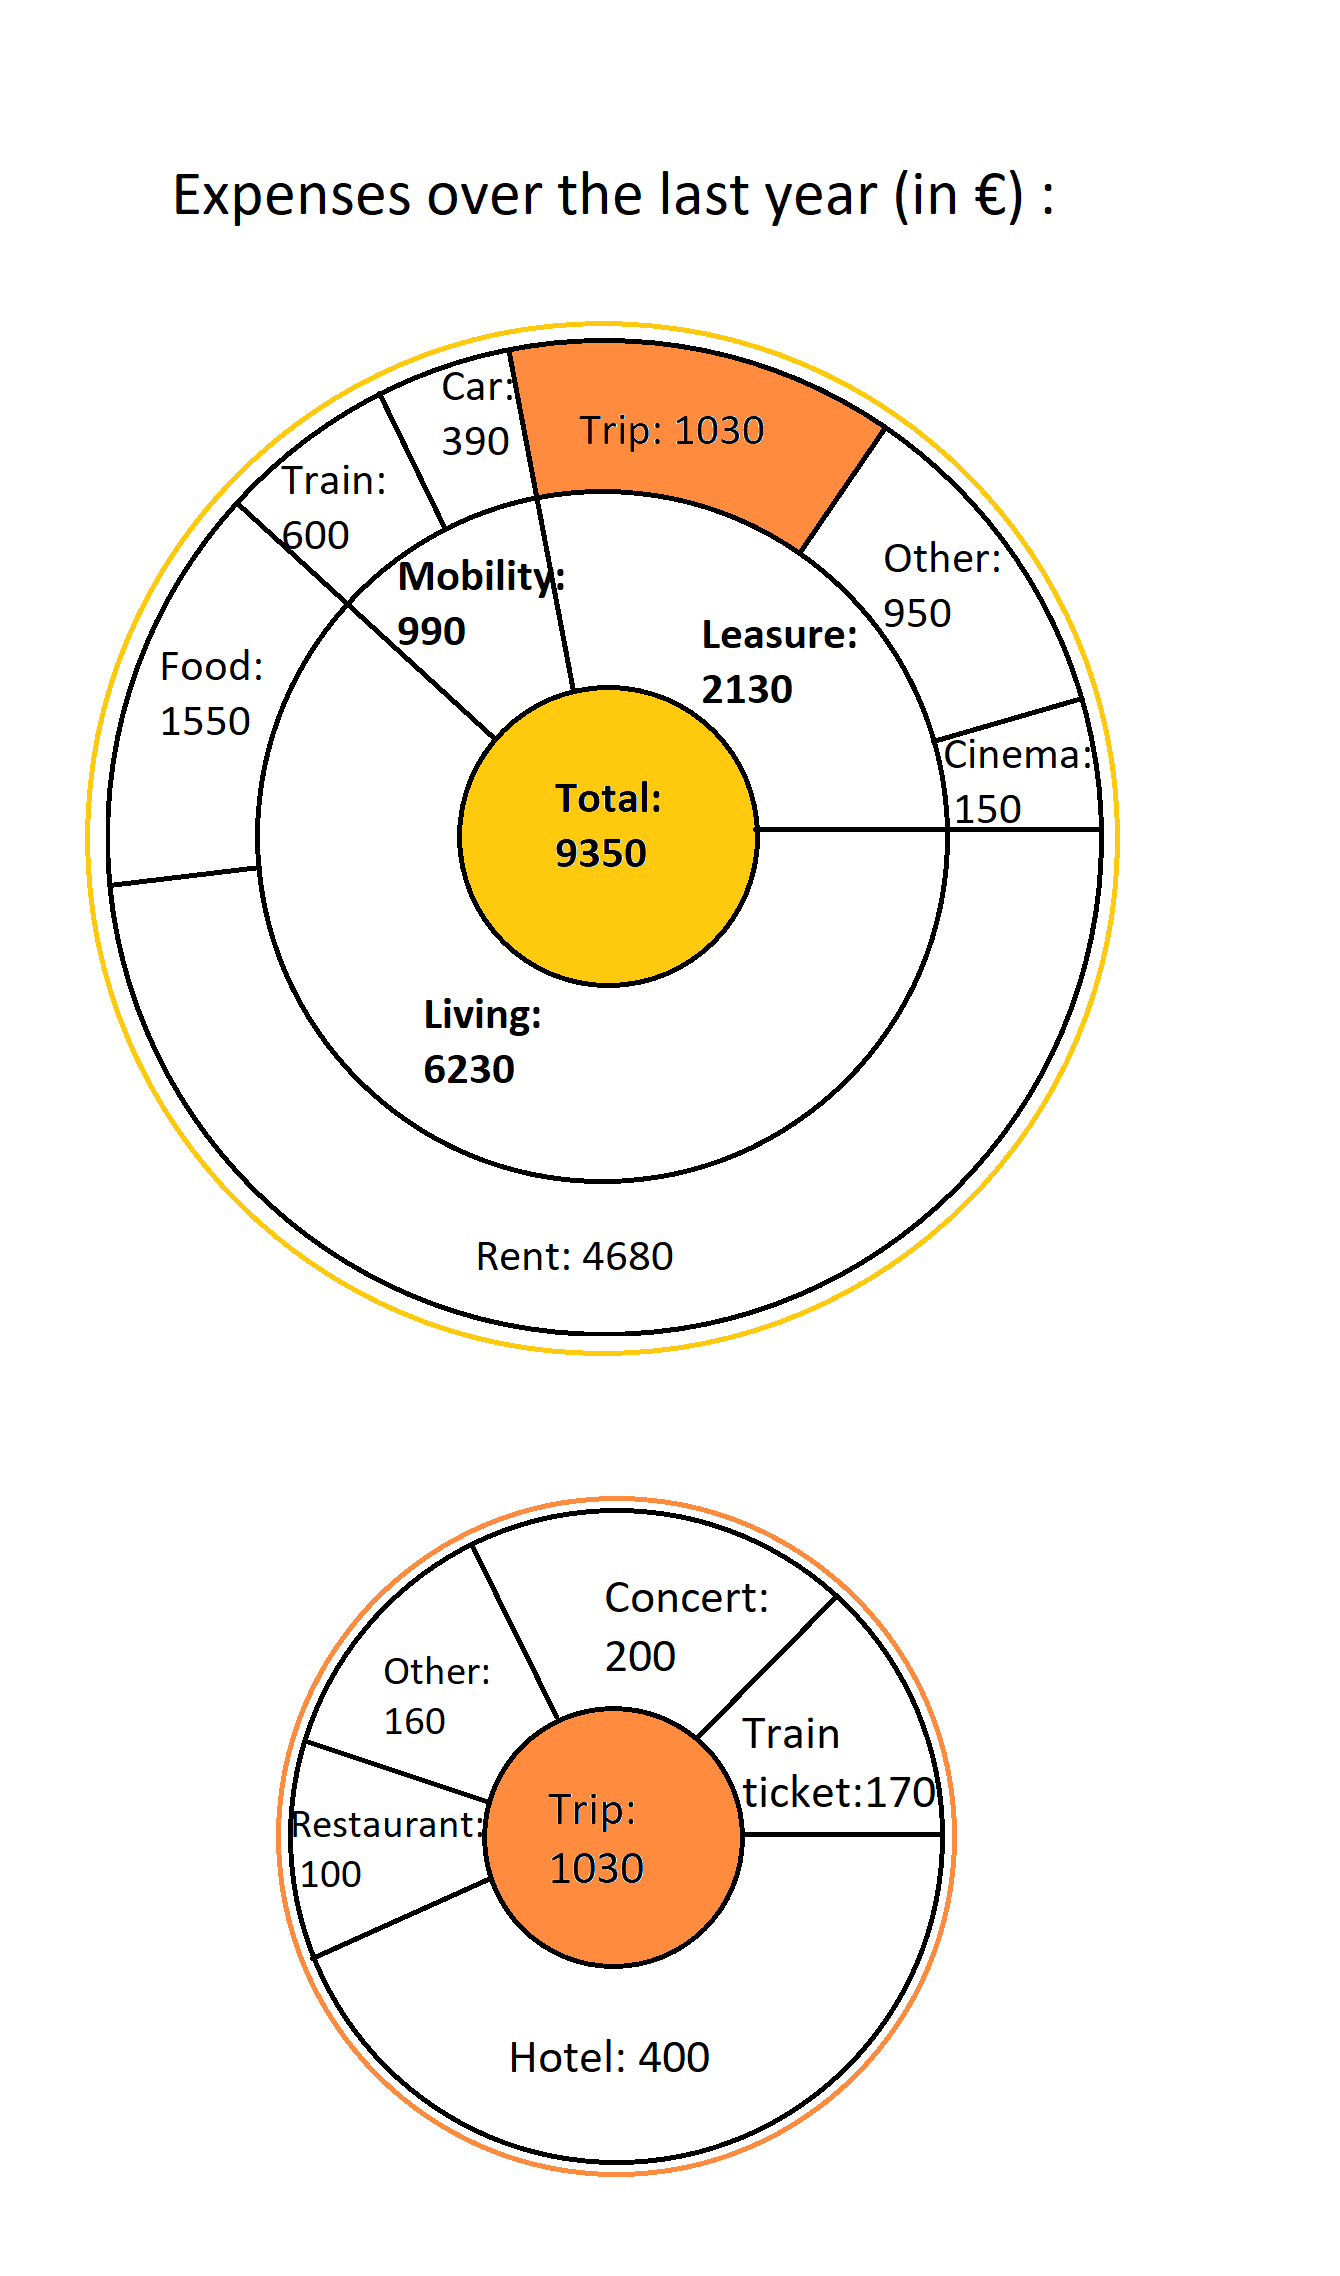
\includegraphics[width=0.8\linewidth]{expenses.png}\\
We elected to use a stacked tree as with this kind of representation, weights of nodes can be illustrated by the area they occupy which makes it easier to compare them. The decision to use a radial layout was made because the drawback of distorted areas of nodes of different levels does not really come into play as a user would usually compare nodes of the same level. Since all leaf nodes have the same level, the tree will allways completely fill the cirle, meaning data is represented quite compactly. While a nesting tree would satisfy this as well, it would make it hard to determine parent nodes, a rather important ability for our usecase.
Each specific category can be inspected more closely by selecting them, at which point another stacked tree representing the exact expenses of this category is displayed. While individual expenses of different categories become harder to compare with this representation, we avoid adding another layer to the circle which would quickly become cluttered and hard to read and therefore reduce scalability. Another reason for this layout is that two smaller circles make much more efficient use of the 16:9 aspect ratio than one big circle. The coloring is meant to show that the second grap represents the subtree of the highlighted node.

\section*{Task 2 - Tree-Maps with Slice \& Dice}
\begin{figure}[!ht]
	\centering
	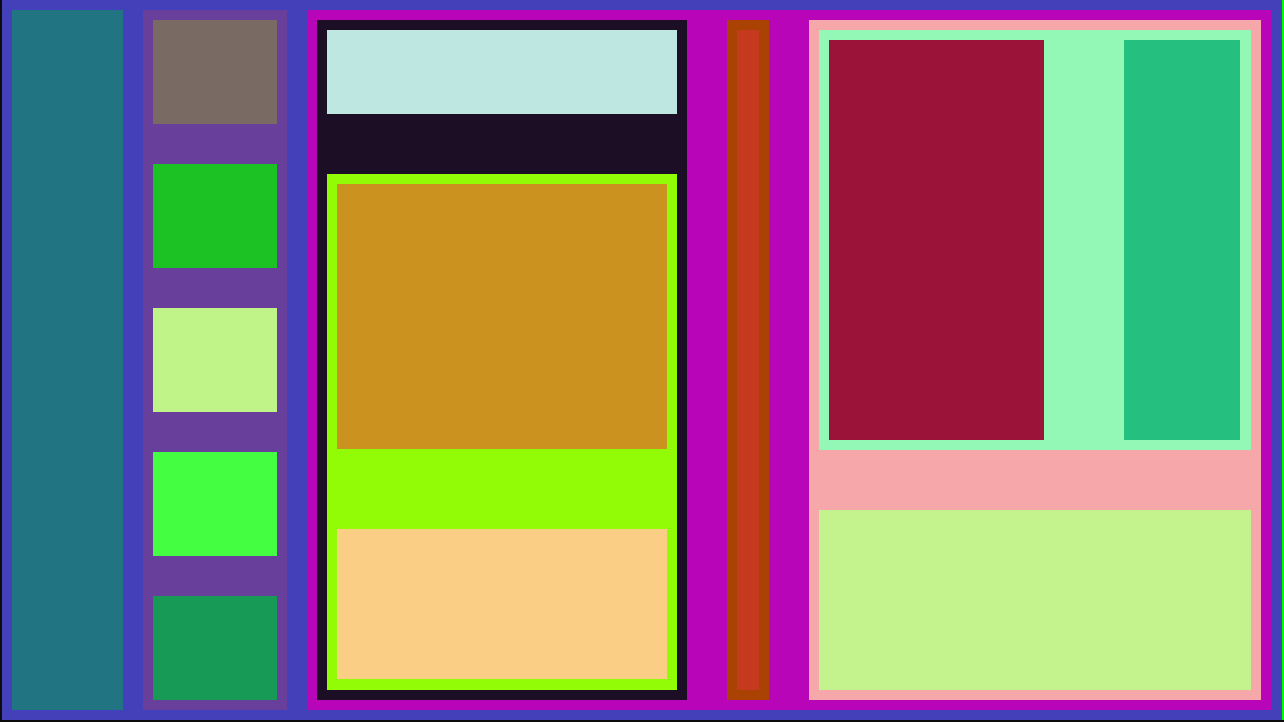
\includegraphics[width=0.9\linewidth]{5_2}
	\caption{Solution}
\end{figure}


\end{document}
